\documentclass[14pt,a1paper,landscape]{tikzposter}

%% Tikzposter is highly customizable: please see
%% https://bitbucket.org/surmann/tikzposter/downloads/styleguide.pdf

%% Available themes: see also
%% https://bitbucket.org/surmann/tikzposter/downloads/themes.pdf
% \usetheme{Default}
% \usetheme{Rays}
% \usetheme{Basic}
% \usetheme{Simple}
 \usetheme{Envelope}
% \usetheme{Wave}
% \usetheme{Board}
% \usetheme{Autumn}
% \usetheme{Desert}

%% Further changes to the title etc is possible
% \usetitlestyle{Default}
% \usetitlestyle{Basic}
 \usetitlestyle{Empty}
% \usetitlestyle{Filled}
% \usetitlestyle{Envelope}
% \usetitlestyle{Wave}
% \usetitlestyle{verticalShading}


\usetikzlibrary{positioning}
\usepackage[utf8]{inputenc}
\usepackage{listingsutf8}
\usepackage{xcolor}
%\usepackage[edges]{forest}
\usepackage [sfdefault]{cabin}
\usepackage[T1]{fontenc}
\usepackage{natbib}
\usepackage{wrapfig}
\definecolor{mymauve}{rgb}{0.58,0,0.82}

\author{Eric Rexstad, David L. Miller, Laura Marshall and Len Thomas}
\title{\parbox{0.53\linewidth}{\centering Migrating distance sampling projects from Distance for Windows to the Distance R package}}
\institute{Centre for Research into Ecological and Environmental Modelling University of St Andrews}

%% Uncomment to switch off tikzposter footer
\tikzposterlatexaffectionproofoff

%%%%%%%%%%%%%%%  Yet another multi-logo title solution from THIS WORKS after adding \usetikzlibrary{positioning}
% https://tex.stackexchange.com/questions/263563/add-logos-beyond-the-title-tikzposter

\makeatletter
\newcommand\insertlogoi[2][]{\def\@insertlogoi{\includegraphics[#1]{#2}}}
\newcommand\insertlogoii[2][]{\def\@insertlogoii{\includegraphics[#1]{#2}}}
\newcommand\insertlogoiii[2][]{\def\@insertlogoiii{\includegraphics[#1]{#2}}}
\newcommand\insertlogoiv[2][]{\def\@insertlogoiv{\includegraphics[#1]{#2}}}
\newlength\LogoHSep
\newlength\LogoVSep

\setlength\LogoHSep{60pt}
\setlength\LogoVSep{1cm}

\insertlogoi[width=7cm]{ISEC_Logo_light_background_RGB.png}
\insertlogoii[width=7cm]{CREEM_Logo_trans.png}
\insertlogoiii[width=5.5cm]{02-foundation-vertical-white.png}
\insertlogoiv[width=5cm]{websitelogo_transparent.png}

\renewcommand\maketitle[1][]{  % #1 keys
	\normalsize
	\setkeys{title}{#1}
	% Title dummy to get title height
	\node[transparent,inner sep=\TP@titleinnersep, line width=\TP@titlelinewidth, anchor=north, minimum width=\TP@visibletextwidth-2\TP@titleinnersep]
	(TP@title) at ($(0, 0.5\textheight-\TP@titletotopverticalspace)$) {\parbox{\TP@titlewidth-2\TP@titleinnersep}{\TP@maketitle}};
	\draw let \p1 = ($(TP@title.north)-(TP@title.south)$) in node {
		\setlength{\TP@titleheight}{\y1}
		\setlength{\titleheight}{\y1}
		\global\TP@titleheight=\TP@titleheight
		\global\titleheight=\titleheight
	};
	
	% Compute title position
	\setlength{\titleposleft}{-0.5\titlewidth}
	\setlength{\titleposright}{\titleposleft+\titlewidth}
	\setlength{\titlepostop}{0.5\textheight-\TP@titletotopverticalspace}
	\setlength{\titleposbottom}{\titlepostop-\titleheight}
	
	% Title style (background)
	\TP@titlestyle
	
	% Title node
	\node[inner sep=\TP@titleinnersep, line width=\TP@titlelinewidth, anchor=north, minimum width=\TP@visibletextwidth-2\TP@titleinnersep]
	at (0,0.5\textheight-\TP@titletotopverticalspace)
	(title)
	{\parbox{\TP@titlewidth-2\TP@titleinnersep}{\TP@maketitle}};
	
	\node[inner sep=0pt,anchor=west]
	at ([shift={(-\LogoHSep,\LogoVSep)}]title.west)
	(logo1)
	{\@insertlogoi};
	
	\node[inner sep=0pt,anchor=west,right=of logo1] 
	(logo2)
	{\@insertlogoii};
	
	\node[inner sep=0pt,anchor=east] 
	at ([shift={(\LogoHSep,\LogoVSep)}]title.east)
	(logo4)
	{\@insertlogoiv};
	
	\node[inner sep=0pt,left=of logo4] 
	(logo4)
	{\@insertlogoiii};
	
	% Settings for blocks
	\normalsize
	\setlength{\TP@blocktop}{\titleposbottom-\TP@titletoblockverticalspace}
}
\makeatother

%%%%%%%%%%%%%%%%%%%%%%%%%%%%%%%%%%%%%%%%%%   

\begin{document}
\maketitle

\begin{columns}

\column{0.333}

\block{Introduction}{
The Distance software \citep{thomas_distance_2010} has been downloaded >40,000 times in its 20-year history.   It consists of a Windows-based Graphical User Interface (GUI) that gives users ready access to survey design tools (written in Visual Basic) and analysis engines (written in FORTRAN and, more recently, R). For some users, there my be benifits to performing their analyses directly with the underlying R code, rather than working with the GUI.
	\begin{tikzfigure}%[Traditional Distance for Windows interface (left) and distance sampling analysis in R (right).]
		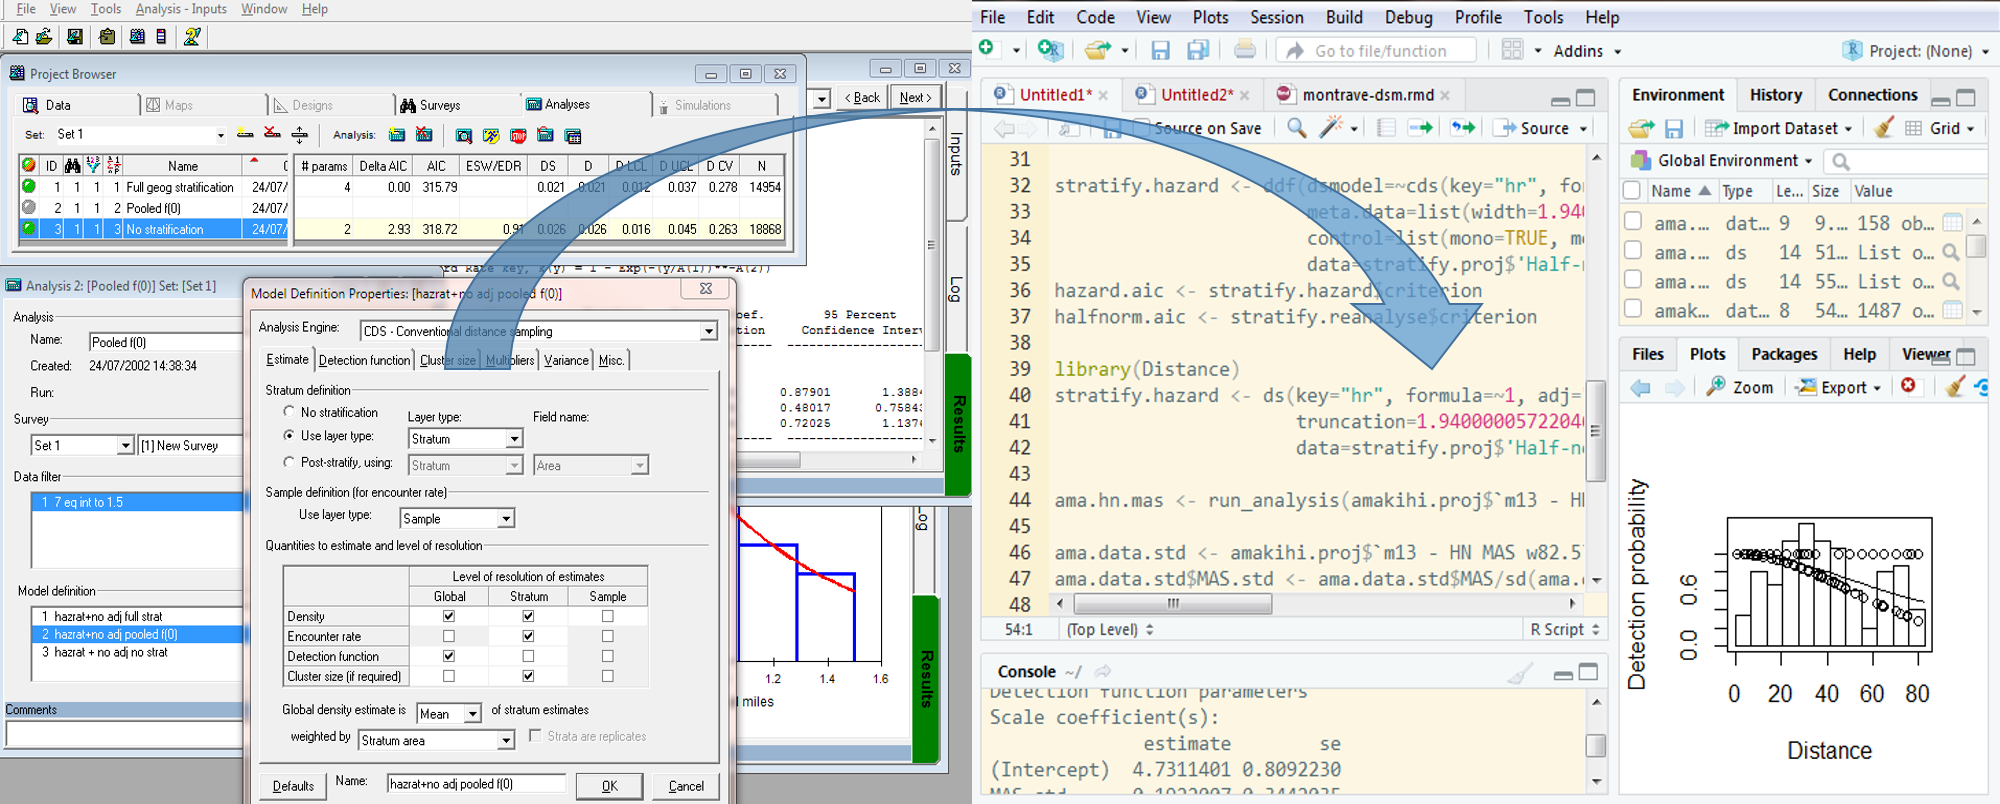
\includegraphics[width=0.95\linewidth]{merged-grabs.png}
	\end{tikzfigure}

Challenges hindering the transition between analysis with the GUI and analyses in R are two-fold:
\begin{itemize}
	\item Legacy data reside in Distance (GUI) projects, unavailable for importing into R, and
	\item Analyses that are easily described using the GUI may be difficult to specify, particularly if analyst is not proficient in R.
\end{itemize}
}

\note[rotate=8, connection, width = 7cm, % targetoffsety=-2cm,
% roundedcorners=15, targetoffsetx=2cm
]{How to make this transition?}

\block{Getting data out of Distance}{

\begin{wrapfigure}[10]{l}{0.6\linewidth}
	\begin{tikzfigure}
		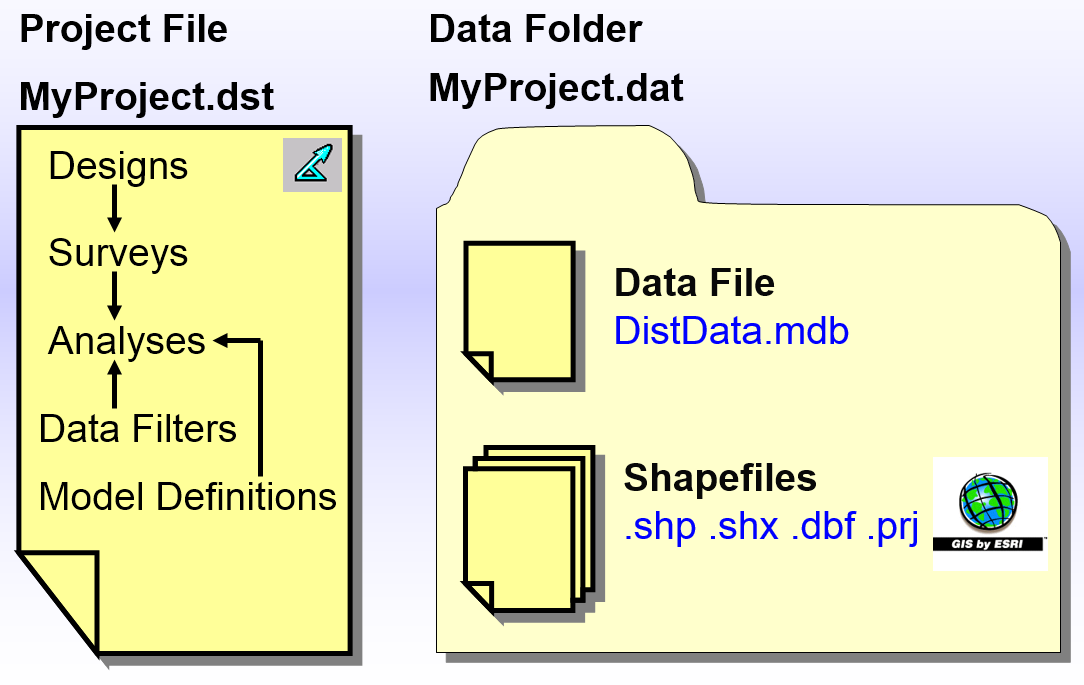
\includegraphics[width=.85\linewidth]{dst-file-structure.PNG}
	\end{tikzfigure}
\end{wrapfigure}

Distance sampling analysis are defined in Distance project files (an Access database).

\begin{itemize}
	\item Data
	\item Model definitions
	\item Analysis results
\end{itemize}

\texttt{readdst} uses \texttt{RODBC} (Windows, the 32-bit version of R must be used for RODBC to function properly) or \texttt{mdb-tools} (Mac) to mine the information from the database.  With the database components available, a sequence of translation steps are undertaken.

\begin{itemize}
	\item Translate model definitions into R code
	\item Save data into an R \texttt{environment}
	\item Extract results from the database for completed analyses
\end{itemize}

}

\column{0.3333}
\block{Converting Distance projects to R}
{
	Workhorse function in \texttt{readdst} package is \texttt{convert\_projects()}.  Its single argument is simply the path to an existing Distance GUI project (created by Distance 6 or 7).  \texttt{convert\_projects()} interrogates the Access database and translates the contents of database tables into an R object of class \texttt{converted\_distance\_analyses}, a list of lists of class \texttt{converted\_distance\_analysis}.
}
	
%	
%\block{}
%{
%	
%% https://tex.stackexchange.com/questions/23647/drawing-a-directory-listing-a-la-the-tree-command-in-tikz	
%\begin{tikzfigure}[Structure of object produced by \texttt{convert\_project()}.]
%	\label{fig:object}
%\begin{forest}
%	for tree={%
%		font=\footnotesize,
%		folder,
%		grow'=0,
%		fit=tight,
%	}
%	[analysis\_object
%	[call
%	]
%	[aic.select
%	]
%	[status
%	]
%	[env%,  label=right:where data reside
%	[data]
%	[obs.table]
%	[region.table]
%	[sample.table]
%	[units]
%	]
%	[filter]
%	[group\_size
%%	[Bias]
%%	[by]
%	]
%	[detection\_by]
%	[gof\_intervals]
%	[estimation
%%	[by]
%%	[Design]
%%	[Weight]
%	]
%	[ID]
%	[engine]
%	[project]
%	[project\_file]
%	]
%\end{forest}
%\end{tikzfigure}
%}


\block{Object produced by \texttt{convert\_project()}}
{
	
	The list returned by \texttt{convert\_project()}, for a given entry (analysis), contains all the salient information of a Distance analysis extracted from the Access database.  We point out two elements of the list critical to subsequent processing of the now-extracted data.
	\begin{description}
		\item [call] R code call to the function \texttt{ddf()} in package \texttt{mrds} to duplicate the analyses done in the Distance GUI.
		\item [env] An \textit{environment} consisting of a set of data frames.  These data frames include the original data extracted from the Distance project, along with the observation, sample and region tables describing the hierarchial nature of the data base.
	\end{description}
	
	The \texttt{converted\_distance\_analysis} list can be passed as an argument to \texttt{run\_analysis()}.  Given \texttt{object} has been created by a call to \texttt{convert\_project}, \texttt{run\_analysis()} will perform an \texttt{mrds} analysis by processing data in \texttt{object\$env} using \texttt{ddf()} syntax in \texttt{object\$call} to conduct a distance sampling analysis.
} 


\block{Learning distance sampling in R}
{
	Distance GUI users can use \texttt{converted\_distance\_analysis} objects to learn how to perform corresponding analyses using the \texttt{mrds} R package:
	%%%  fix to code inside block error -- https://tex.stackexchange.com/questions/228675/how-can-i-put-a-code-listing-in-a-tikzposter-block
		
		\lstset{backgroundcolor=\color{white}, keywordstyle=\color{blue}, stringstyle=\color{mymauve},
		        inputencoding=utf8, extendedchars=true}
	    \lstinputlisting[fontadjust]{convert-stratify.r}
	
	Note too that components from objects of type \texttt{converted\_distance\_analysis} can be analysed using the \texttt{ds()} function from the \texttt{Distance} package.
}


\column{0.3333}

\block{Comparative analysis of data sets}{
	
	The \texttt{test\_stats()} function in \texttt{readdst} performs the analysis residing in the call element of the \texttt{converted\_distance\_analysis}, producing estimates of parameters of distance sampling analyses (\emph{e.g.} AIC scores, $\hat{P}_a$, $\hat{D}$, $\hat{D}$ and associated measures of precision).  These results are contrasted with estimates of the same parameters stored in the Access data base, as computed by the Distance GUI.
	
	The resulting comparison is produced in tabular form with the difference between estimates presented as proportions.  Those comparative estimates within a specified tolerance are designated with \textbf{X}.
	\lstset{backgroundcolor=\color{white}, keywordstyle=\color{blue}, stringstyle=\color{mymauve}, basicstyle=\normalsize}
	\lstinputlisting[fontadjust]{stat-table.txt}
	
	This testing capability is part of our strategy to migrate software development from the existing Distance GUI to R packages.  We can check consistency of results between the Distance GUI and developing R code.
}

\block{Caveats}{
	\texttt{readdst} is not able to translate all GUI analyses into R code.  Current limitations are inability to translate
	\begin{itemize}
		\item analyses using the \texttt{dsm}, \texttt{mads} and \texttt{Dssim} engines,
		\item analyses using post-stratification and
		\item bootstrapping for variance estimation.
	\end{itemize}
}

\block{Additional information}{

	\coloredbox[bgcolor=lightgray, framecolor=black]{
		\nocite{*} % Insert publications even if they are not cited in the poster
		\small{\bibliographystyle{humannat}
			\bibliography{isecposter}}
	}
	
	\begin{tikzfigure}
		
\includegraphics[width=.16\linewidth]{qrcode-readdst.png}
		
\includegraphics[width=.16\linewidth]{QRcap-readdst.png}
		\includegraphics[width=.16\linewidth]{qrcode-bioRxiv.png}
		
\includegraphics[width=.16\linewidth]{QRcap-bioRxiv.png}
		
\includegraphics[width=.16\linewidth]{qrcode-thomas-1e5687.png}
		
\includegraphics[width=.16\linewidth]{QRcap-thomasetal.png}	
	\end{tikzfigure}
}

\end{columns}


\end{document}
